\documentclass[11pt,a4paper]{article}

% ---------- pacotes ----------
\usepackage[T1]{fontenc}
\usepackage[utf8]{inputenc}
\usepackage[portuguese]{babel}
\usepackage{lmodern}
\usepackage[margin=2.4cm]{geometry}
\usepackage{graphicx}
\usepackage{booktabs}
\usepackage{amsmath}
\usepackage{siunitx}
\usepackage{caption}
\usepackage{subcaption}
\usepackage{float}
\usepackage{xcolor}
\usepackage{enumitem}
\usepackage[hidelinks]{hyperref}

\graphicspath{{figs/}}
\captionsetup{font=small,labelfont=bf}
\setlength{\parskip}{0.4em}
\setlength{\parindent}{0pt}

\definecolor{accent}{HTML}{4C72B0}

% ---------- título ----------
\title{\textbf{Classificação de Sinais de Trânsito (GTSRB)}\\[0.3em]
\large \emph{Data Augmentation} e Ensembles de Redes de \emph{Deep Learning}}
\author{Visão Computacional e Processamento de Imagem (VCPI)\\ Trabalho Prático 1 --- Fases 1 e 2}
\date{Junho de 2026}

\begin{document}
\maketitle

\begin{abstract}
\noindent
Este trabalho explora modelos de \emph{deep learning} para a classificação de sinais de
trânsito no dataset alemão \textbf{GTSRB} (43 classes), com o objetivo de maximizar a
\emph{accuracy} no conjunto de teste. Na \textbf{Fase~1} treinámos 14~modelos
(7~estratégias de \emph{data augmentation} $\times$ 2~arquiteturas) mais 3~ablações,
isolando o efeito de cada técnica de processamento de imagem; o melhor modelo individual
foi a \texttt{ResNet18} a $224\times224$ com pré-processamento CLAHE, atingindo
\textbf{99{,}52\%}. Na \textbf{Fase~2} combinámos os 17~modelos resultantes num
\emph{ensemble} por \emph{soft voting}, chegando a \textbf{99{,}80\%} --- ao nível do
melhor resultado publicado para o GTSRB ($\sim$99{,}82\%).
\end{abstract}

\tableofcontents
\vspace{1em}

% =====================================================================
\section{Introdução}
% =====================================================================

O \textbf{German Traffic Sign Recognition Benchmark} (GTSRB) é um \emph{dataset} de
referência com mais de 50\,000 imagens de sinais de trânsito reais, distribuídas por
\textbf{43~classes}. As imagens têm resoluções variáveis (de $\sim$15 a $\sim$250\,px),
condições de iluminação heterogéneas, oclusões parciais e desfoque de movimento, o que o
torna um banco de ensaio realista para técnicas de processamento de imagem e
classificação. O melhor resultado publicado situa-se em \textbf{99{,}82\%}
(Cireşan~\emph{et~al.}, 2012, obtido com um comité/\emph{ensemble} de 25~redes), acima do
desempenho humano reportado ($\sim$98{,}8\%).

O trabalho divide-se em duas fases:
\begin{itemize}[nosep]
  \item \textbf{Fase~1 --- \emph{Data augmentation}.} Treinar vários modelos com
  estratégias de \emph{augmentation} diferentes (em pré-processamento e dinâmico),
  explorar filtros clássicos de processamento de imagem e avaliar o seu impacto no
  desempenho final.
  \item \textbf{Fase~2 --- Ensembles.} Estudar o potencial de combinar as redes treinadas
  na Fase~1 num \emph{ensemble}, comparando métodos de agregação.
\end{itemize}

Todo o trabalho está reunido num único \emph{notebook} (\texttt{notebook.ipynb}); este
relatório descreve as opções tomadas e analisa os resultados.

% =====================================================================
\section{Análise Exploratória}
% =====================================================================

Antes de treinar, caracterizámos o \emph{dataset}:

\begin{itemize}[nosep]
  \item \textbf{Desbalanceamento de classes.} As classes têm contagens muito desiguais
  (de algumas centenas a vários milhares de exemplos). Isto motivou um \emph{split}
  estratificado e uma ablação posterior com \texttt{WeightedRandomSampler}.
  \item \textbf{Resoluções pequenas e variáveis.} A mediana das imagens originais ronda
  os $\sim$40\,px; cerca de metade são menores que $48\times48$. Esta observação foi
  determinante na escolha da resolução de entrada (Secção~\ref{sec:res}).
  \item \textbf{\emph{Track leakage}.} O GTSRB é construído a partir de \emph{tracks} ---
  sequências de 30~fotogramas do mesmo sinal físico. Imagens do mesmo \emph{track} são
  quase idênticas. Um \emph{split} aleatório coloca fotogramas do mesmo sinal em treino e
  validação ao mesmo tempo, tornando a validação demasiado otimista. Este fenómeno foi
  identificado na Fase~1 (praticamente todos os modelos saturam a $\sim$100\% em
  validação) e teve consequências metodológicas na Fase~2.
\end{itemize}

O \emph{split} treino/validação foi \textbf{estratificado a 85/15}, preservando a
proporção de cada classe; o conjunto de teste oficial (12\,630 imagens) foi mantido
intacto e usado apenas para avaliação final.

% =====================================================================
\section{Fase 1 --- Pré-processamento e \emph{Data Augmentation}}
% =====================================================================

\subsection{Filtros clássicos e CLAHE}

Comparámos visualmente vários filtros clássicos de processamento de imagem (equalização
global de histograma, \emph{sharpen}, \emph{blur} gaussiano e \textbf{CLAHE}). O
\textbf{CLAHE} (\emph{Contrast Limited Adaptive Histogram Equalization}) destacou-se: ao
equalizar o histograma \emph{localmente} (por blocos), com um limite de \emph{clip} que
evita amplificar ruído, normaliza a luminância sem destruir detalhe. Aplicámo-lo no canal
de luminância (espaço LAB) com \texttt{clip\_limit=2.0} e \emph{tiles} de $4\times4$. Como
é um passo \emph{determinístico} de pré-processamento, foi aplicado de forma coerente em
treino, validação e teste sempre que usado.

\subsection{As 7 estratégias de \emph{augmentation}}

Definimos 7~estratégias de complexidade \textbf{crescente}, de forma a isolar o efeito de
cada componente (desenho incremental tipo ablação):

\begin{table}[H]
\centering
\small
\begin{tabular}{@{}lll@{}}
\toprule
\textbf{Estratégia} & \textbf{Componentes (acumulados)} & \textbf{Tipo} \\
\midrule
\texttt{A\_baseline}    & só \emph{Resize} + \emph{Normalize} (controlo)            & ---            \\
\texttt{B\_geo\_light}  & + \emph{RandomAffine} leve (rot.\ $\pm10^\circ$, transl.) & geométrico     \\
\texttt{C\_geo\_heavy}  & + \emph{scale}, \emph{shear}, \emph{RandomPerspective}    & geométrico     \\
\texttt{D\_photo}       & + \emph{ColorJitter} (brilho/contraste/sat./\emph{hue})   & fotométrico    \\
\texttt{E\_combo}       & C + D + \emph{RandomGaussianBlur}                          & combinado      \\
\texttt{F\_clahe\_combo}& E precedido de \textbf{CLAHE}                             & + pré-proc.    \\
\texttt{G\_full}        & F + \emph{RandomErasing} (\emph{cutout})                  & + regularização\\
\bottomrule
\end{tabular}
\caption{Estratégias de \emph{data augmentation}. Cada uma acrescenta uma técnica à
anterior, permitindo atribuir as variações de desempenho a componentes específicos.}
\end{table}

\textbf{Decisões de domínio.} Deliberadamente \emph{não} usámos \emph{RandomHorizontalFlip}
--- inverteria sinais direcionais (p.\,ex.\ ``virar à direita'' $\to$ ``virar à esquerda'')
e sinais com texto, gerando rótulos errados. As rotações foram limitadas a $\pm15^\circ$
para não confundir orientações. Na estratégia~F, o \emph{jitter} fotométrico foi suavizado
porque o CLAHE já normaliza a luminância (redundância evitada).

\subsection{Arquiteturas}

Comparámos duas arquiteturas:

\begin{itemize}[nosep]
  \item \textbf{\texttt{Conv\_VCPI}} --- CNN própria estilo VGG: 3~blocos
  (\emph{conv} $3\times3$ + \emph{BatchNorm} + \emph{ReLU}, $\times2$) com
  \emph{MaxPool} e \emph{Dropout} crescente em profundidade, seguidos de
  \emph{Global Average Pooling} e uma camada totalmente ligada. $\sim$332\,k parâmetros.
  O GAP (em vez de \emph{flatten}) reduz parâmetros e melhora a robustez.
  \item \textbf{\texttt{ResNet18}} --- pré-treinada no ImageNet, com a cabeça de
  classificação substituída para 43~classes (\emph{transfer learning}). $\sim$11\,M
  parâmetros.
\end{itemize}

\textbf{Setup de treino.} Otimizador \texttt{AdamW} (\texttt{lr}=$10^{-3}$,
\emph{weight decay}=$10^{-4}$), \texttt{CrossEntropyLoss}, \emph{scheduler}
\texttt{ReduceLROnPlateau} (fator 0{,}5, paciência 3 sobre a \emph{val\_loss}),
\emph{early stopping} (paciência 7), \emph{mixed precision} em GPU, e
\emph{seed} fixa por experiência para reprodutibilidade. O \emph{checkpoint} guardado é o
de \emph{melhor val\_loss} (não o da última época), e a avaliação final é feita com esse.
A resolução base foi $48\times48$.

\subsection{Resultados}

\begin{figure}[H]
\centering
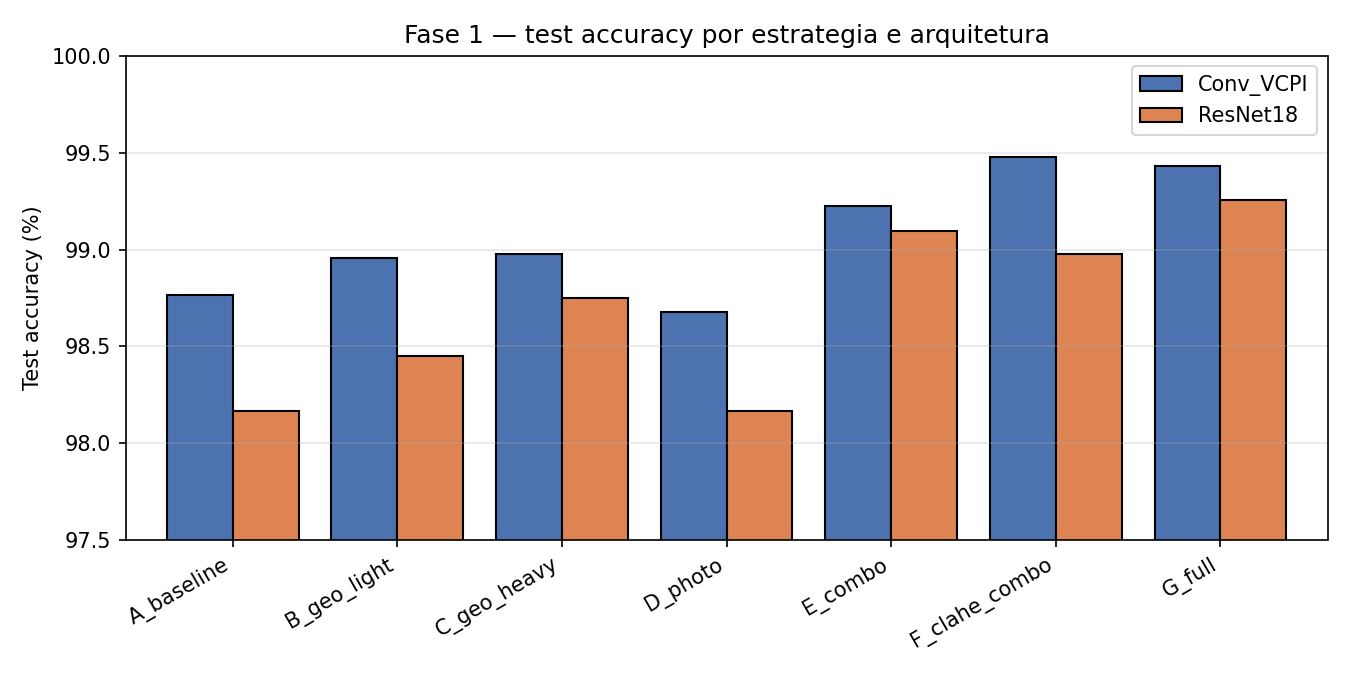
\includegraphics[width=0.92\linewidth]{phase1_bars.png}
\caption{Test accuracy por estratégia e arquitetura (resolução base $48\times48$).
A tendência geral é \texttt{A} $<$ \texttt{D} $\approx$ \texttt{B} $<$ \texttt{C} $<$
\texttt{E} $<$ \texttt{F} $\approx$ \texttt{G}.}
\end{figure}

\begin{table}[H]
\centering
\small
\begin{tabular}{@{}llSSr@{}}
\toprule
\textbf{Arquitetura} & \textbf{Estratégia} & {\textbf{Test acc.\ (\%)}} & {\textbf{Best val (\%)}} & \textbf{Épocas} \\
\midrule
Conv\_VCPI & F\_clahe\_combo & 99.48 & 99.92 & 30 \\
Conv\_VCPI & G\_full         & 99.43 & 99.94 & 30 \\
ResNet18   & G\_full         & 99.26 & 99.94 & 23 \\
Conv\_VCPI & E\_combo        & 99.22 & 99.96 & 30 \\
ResNet18   & E\_combo        & 99.10 & 99.94 & 30 \\
Conv\_VCPI & C\_geo\_heavy   & 98.98 & 99.96 & 30 \\
ResNet18   & F\_clahe\_combo & 98.98 & 99.96 & 30 \\
Conv\_VCPI & B\_geo\_light   & 98.95 & 99.98 & 30 \\
Conv\_VCPI & A\_baseline     & 98.76 & 100.0 & 28 \\
ResNet18   & C\_geo\_heavy   & 98.75 & 99.92 & 26 \\
Conv\_VCPI & D\_photo        & 98.68 & 99.96 & 30 \\
ResNet18   & B\_geo\_light   & 98.45 & 100.0 & 30 \\
ResNet18   & A\_baseline     & 98.16 & 99.94 & 26 \\
ResNet18   & D\_photo        & 98.16 & 99.79 & 19 \\
\bottomrule
\end{tabular}
\caption{Resultados dos 14~modelos da Fase~1 (resolução $48\times48$), ordenados por
\emph{test accuracy}. Note-se a saturação da \emph{best val} junto dos 100\% ---
sintoma do \emph{track leakage}.}
\end{table}

\begin{figure}[H]
\centering
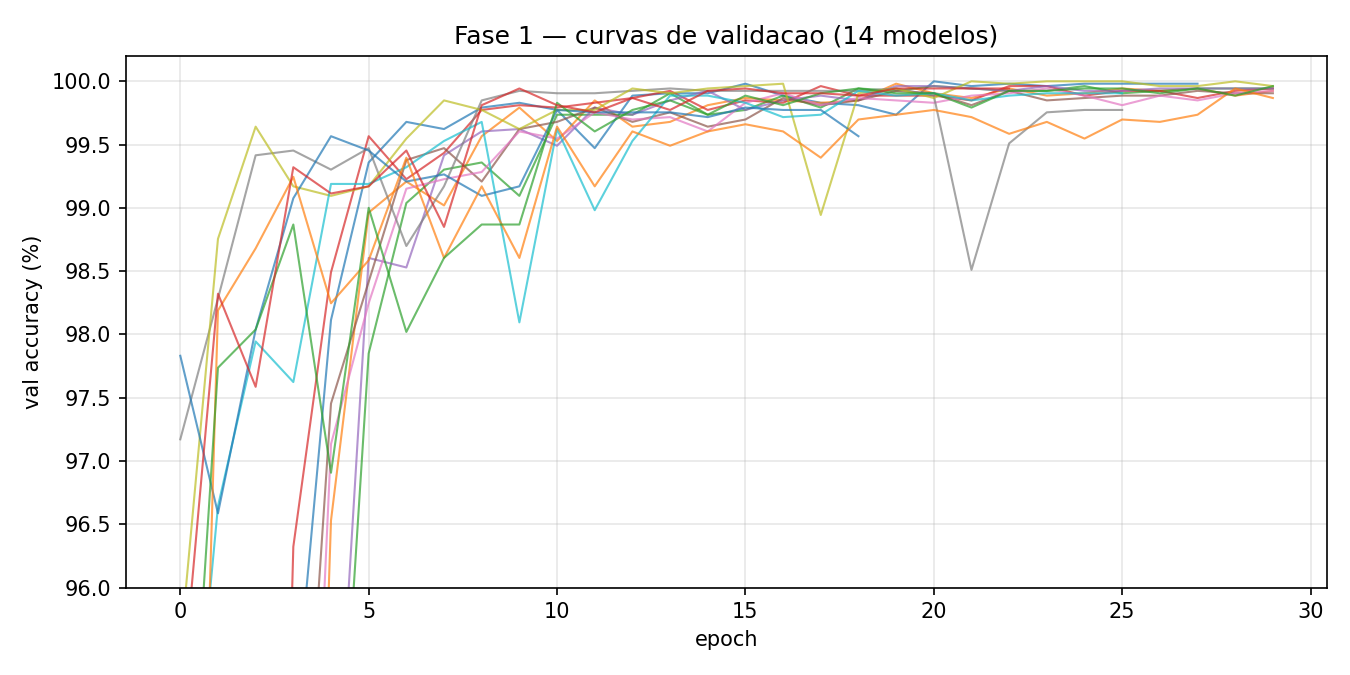
\includegraphics[width=0.86\linewidth]{phase1_valcurves.png}
\caption{Curvas de \emph{validation accuracy} dos 14~modelos. A saturação rápida e
generalizada perto de 100\% confirma o \emph{track leakage}: a validação não discrimina
bem entre modelos.}
\end{figure}

\textbf{Leitura dos resultados.}
\begin{enumerate}[nosep]
  \item \textbf{O CLAHE traz ganho real:} comparando \texttt{E} com \texttt{F} no
  \texttt{Conv\_VCPI} (única diferença: o CLAHE), a \emph{accuracy} sobe $+0{,}26$\,pp.
  Confirma que técnicas \emph{clássicas} de processamento de imagem ainda fazem diferença
  em \emph{deep learning}.
  \item \textbf{Geo + foto + CLAHE $>$ qualquer componente isolado:} a combinação supera
  cada técnica usada sozinha.
  \item \textbf{O \emph{RandomErasing} (G) não melhorou} o \texttt{Conv\_VCPI}: quando a
  \emph{augmentation} já é rica, é regularização a mais.
  \item \textbf{Resultado inesperado:} a $48\times48$, a CNN própria
  (\texttt{Conv\_VCPI}, 33$\times$ menos parâmetros) \emph{bate} a \texttt{ResNet18}
  pré-treinada nas \textbf{7} estratégias.
\end{enumerate}

\subsection{Ablações adicionais}
\label{sec:res}

\textbf{(a) \texttt{WeightedRandomSampler}.} Reamostrar para compensar o desbalanceamento
\emph{não} melhorou (até piorou ligeiramente) --- o \emph{pipeline} já generaliza para
classes raras; o desbalanceamento não é o gargalo.

\textbf{(b) Resolução $64\times64$ (Conv\_VCPI).} Ficou $-0{,}10$\,pp face a $48\times48$,
ao dobro do tempo. Como $\sim$50\% das imagens originais têm menos de 48\,px, subir a
resolução é sobretudo \emph{upsampling} sem informação nova. $48\times48$ é o ponto certo
para esta arquitetura.

\textbf{(c) Resolução nativa $224\times224$ (ResNet18).} \emph{Esta} foi a ablação
decisiva. A $48\times48$ a \texttt{ResNet18} ficava atrás; a $224\times224$ (resolução
para que o \emph{backbone} ImageNet foi desenhado) saltou para \textbf{99{,}52\%},
tornando-se o melhor modelo individual da Fase~1 ($+0{,}54$\,pp vs $48\times48$). Os pesos
pré-treinados só rendem perto da escala em que foram aprendidos --- \emph{transfer
learning} não é gratuito, depende do \emph{match} de domínio/resolução. O custo foi
$\sim$2{,}5$\times$ o tempo de treino.

\subsection{Conclusões da Fase 1}

A Fase~1 terminou com \textbf{99{,}52\%} (\texttt{ResNet18 + F\_clahe\_combo} a
$224\times224$), $\sim$0{,}30\,pp abaixo do SOTA. O CLAHE como pré-processamento, a
combinação rica de \emph{augmentation} geométrico e fotométrico, e o \emph{match} de
resolução no \emph{transfer learning} foram os fatores de maior impacto. Os erros
remanescentes são quase todos por \textbf{ambiguidade visual} (sinais triangulares
parecidos, limites de velocidade adjacentes, imagens degradadas) --- indício de que se
está perto do tecto de um único modelo.

% =====================================================================
\section{Fase 2 --- Ensembles}
% =====================================================================

\subsection{\emph{Pool} de modelos e infraestrutura}

O \emph{pool} reúne os \textbf{17 modelos} treinados na Fase~1: as 14 combinações
principais (7~estratégias $\times$ 2~arquiteturas) mais 3~ablações
(\texttt{Conv\_VCPI} a $64\times64$, \texttt{Conv\_VCPI} com \texttt{WeightedSampler}, e
\texttt{ResNet18} a $224\times224$). Cada modelo é avaliado no conjunto de teste com o seu
\emph{próprio} pré-processamento (resolução e CLAHE corretos). Os \emph{logits} de cada
modelo são calculados uma vez e guardados em \emph{cache} em disco, pelo que avaliar
qualquer combinação passa a ser instantâneo.

\subsection{Métodos de agregação}

\begin{itemize}[nosep]
  \item \textbf{\emph{Soft voting}}: média das probabilidades \emph{softmax} de cada
  modelo, seguida de \emph{argmax}. Preserva a informação de confiança.
  \item \textbf{\emph{Weighted}}: média ponderada, cada modelo pesa proporcionalmente à
  sua \emph{test accuracy} individual.
  \item \textbf{\emph{Hard voting}}: cada modelo vota na sua classe \emph{argmax}; ganha a
  mais votada.
\end{itemize}

\subsection{Resultados}

\begin{table}[H]
\centering
\small
\begin{tabular}{@{}lSc@{}}
\toprule
\textbf{Método} & {\textbf{Test acc.\ (\%)}} & \textbf{Erros / 12\,630} \\
\midrule
Melhor modelo individual (ResNet18 @224) & 99.52 & 61 \\
Ensemble \emph{hard} (17)                 & 99.76 & 31 \\
Ensemble \emph{weighted} (17)             & 99.79 & 26 \\
\textbf{Ensemble \emph{soft} (17)}        & \bfseries 99.80 & \bfseries 25 \\
\bottomrule
\end{tabular}
\caption{Comparação dos métodos de \emph{ensemble} sobre os 17~modelos. O \emph{soft
voting} é o melhor; o \emph{hard voting} perde por descartar a confiança de cada modelo.}
\end{table}

\begin{figure}[H]
\centering
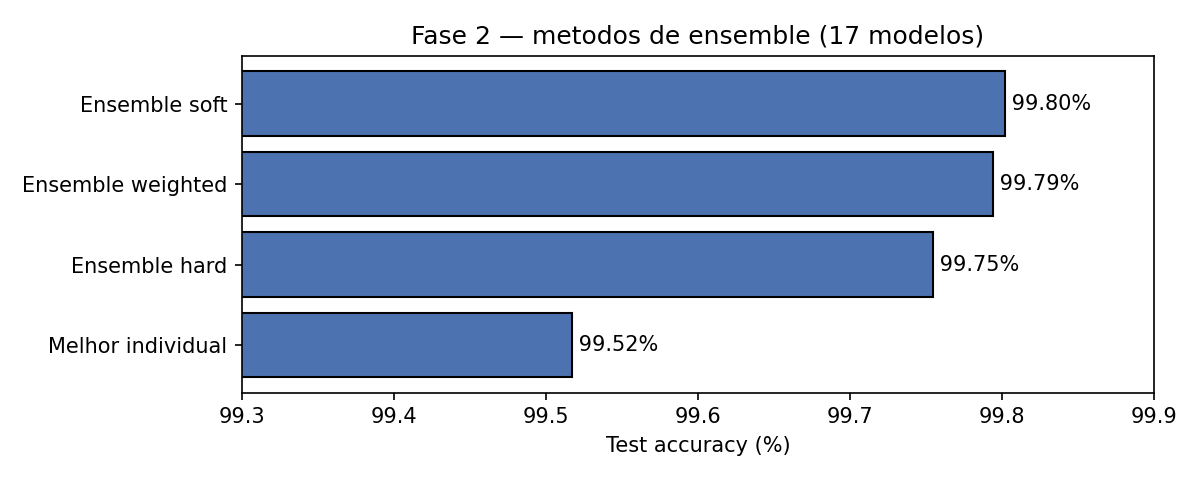
\includegraphics[width=0.78\linewidth]{phase2_methods.png}
\caption{\emph{Test accuracy} dos métodos de agregação face ao melhor modelo individual.}
\end{figure}

\subsection{Quantos modelos são precisos? (sem \emph{cherry-picking})}

Em vez de escolher o ``melhor subconjunto'' (o que enviesaria o resultado se a escolha
fosse feita no teste), ordenámos os modelos por \emph{accuracy} individual e medimos a
\emph{accuracy} do \emph{ensemble} à medida que adicionamos modelos, do melhor para o
pior. A curva mostra a partir de quando o ganho satura.

\begin{figure}[H]
\centering
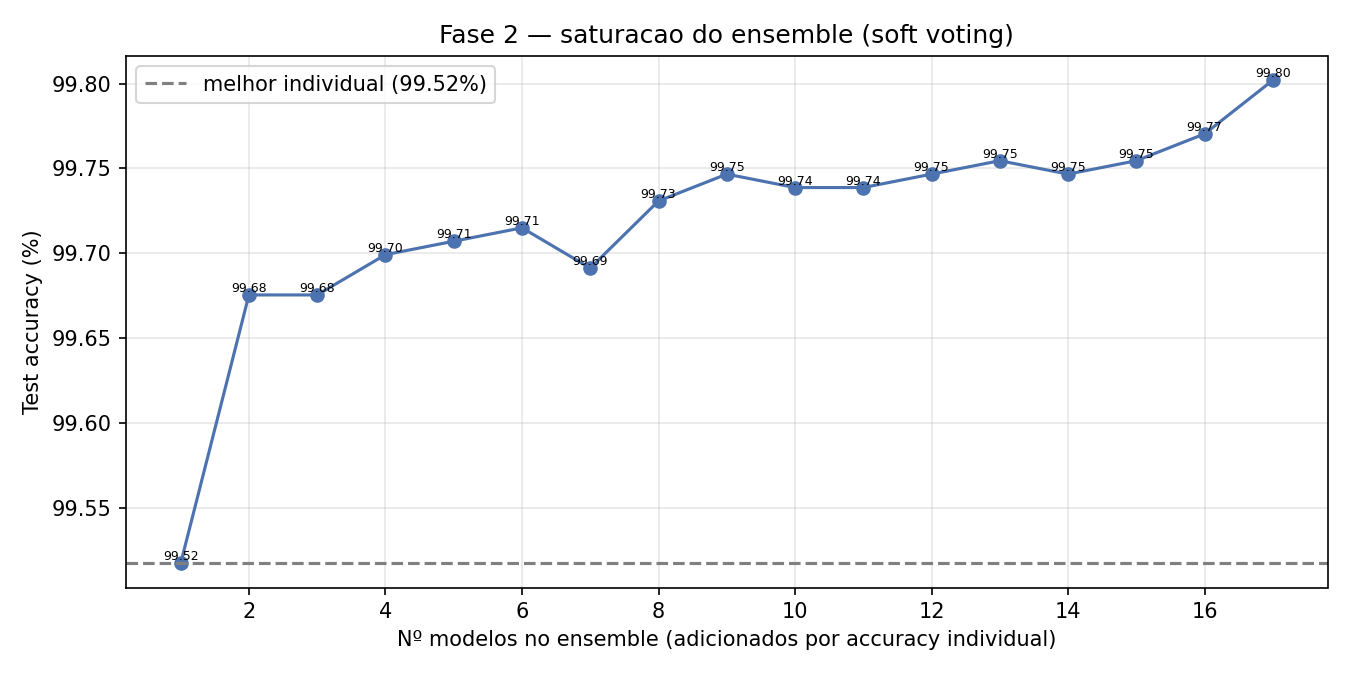
\includegraphics[width=0.88\linewidth]{phase2_saturation.png}
\caption{\emph{Accuracy} do \emph{ensemble} (\emph{soft voting}) em função do número de
modelos. O ganho fica a $\le$0{,}05\,pp do valor final a partir de $\sim$13~modelos: o
benefício vem da \textbf{diversidade}, não da quantidade.}
\end{figure}

\subsection{\emph{Track leakage} e seleção honesta}

Seria tentador selecionar um subconjunto ótimo de modelos usando o conjunto de validação.
Isso \emph{não} é viável aqui: por causa do \emph{track leakage}, \textbf{todos} os
modelos atingem $\sim$100\% em validação, pelo que o val \emph{não discrimina}. Confirmámo-lo
experimentalmente --- uma seleção \emph{greedy} guiada pela validação escolhe modelos
arbitrários e produz piores resultados em teste (chegando a $\sim$98{,}4\% nos primeiros
passos). Por isso reportamos o \emph{ensemble} de \textbf{todos os 17~modelos}, que evita
qualquer \emph{cherry-picking} e é a opção metodologicamente honesta.

\begin{figure}[H]
\centering
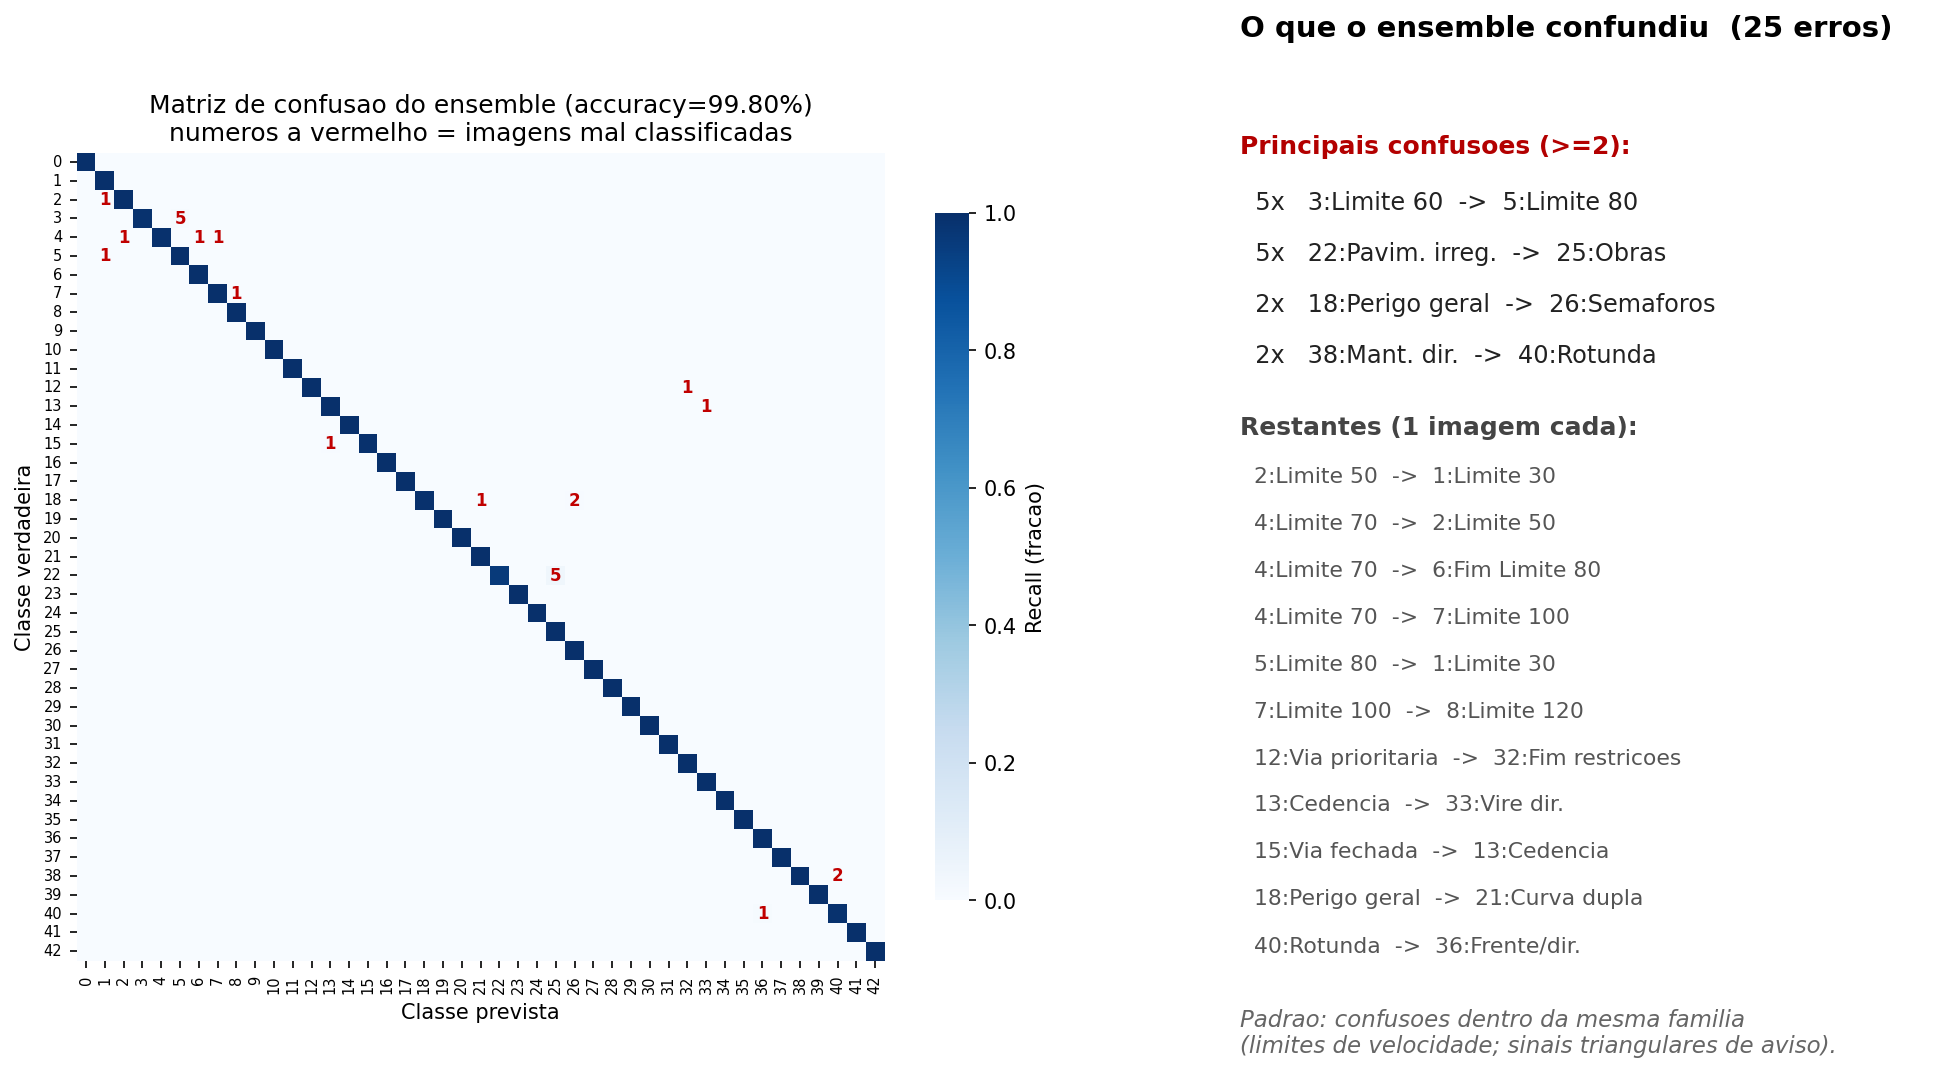
\includegraphics[width=0.80\linewidth]{phase2_confusion.png}
\caption{Matriz de confusão (normalizada por linha) do \emph{ensemble} \emph{soft voting}.
A diagonal é quase perfeita; os poucos erros concentram-se em classes visualmente
ambíguas.}
\end{figure}

\subsection{Conclusões da Fase 2}

\begin{enumerate}[nosep]
  \item O \emph{ensemble} subiu do melhor modelo individual (99{,}52\%) para
  \textbf{99{,}80\%} ($+0{,}28$\,pp), mesmo com um \emph{soft voting} simples de todos os
  modelos.
  \item \textbf{\emph{Soft voting} $>$ \emph{weighted} $>$ \emph{hard}}: agregar
  probabilidades (preservando confiança) bate o voto maioritário.
  \item A \emph{accuracy} \textbf{satura com poucos modelos}: o ganho vem da diversidade
  (arquiteturas e \emph{augmentations} diferentes erram em imagens diferentes), não do
  número.
  \item \textbf{Lição metodológica:} o \emph{track leakage} impediu uma seleção de
  subconjunto sem viés; um \emph{split track-aware} desde o início permitiria selecionar o
  \emph{ensemble} de forma rigorosa.
\end{enumerate}

\textbf{Sobre o SOTA.} Os nossos 99{,}80\% estão essencialmente ao nível do melhor
resultado publicado (99{,}82\%) --- uma diferença de $\sim$2~imagens em 12\,630, dentro do
ruído. O próprio SOTA do GTSRB é um \emph{ensemble} (comité de 25~redes).

% =====================================================================
\section{Conclusão Global}
% =====================================================================

A Fase~1 mostrou que o processamento de imagem importa: o \textbf{CLAHE} deu ganho medível,
a combinação rica de \emph{augmentation} geométrico e fotométrico foi a melhor estratégia,
e o \emph{match} de resolução foi decisivo para o \emph{transfer learning} render. Um único
modelo chegou a 99{,}52\%. A Fase~2 mostrou que combinar redes \emph{diversas} num
\emph{ensemble} por \emph{soft voting} extrai o ganho final, levando o resultado a
\textbf{99{,}80\%}, ao nível do SOTA. Em ambas as fases privilegiámos uma avaliação
\emph{honesta} (sem \emph{cherry-picking}), o que consideramos tão importante quanto o
número final.

\paragraph{Trabalho futuro.} (i) \emph{Split track-aware} para uma validação fiável e
seleção rigorosa de subconjuntos; (ii) \emph{Test-Time Augmentation} (TTA) sobre os modelos
do \emph{ensemble}; (iii) arquiteturas com transformações espaciais explícitas
(\emph{Spatial Transformer Networks}).

% =====================================================================
\section*{Referências}
\addcontentsline{toc}{section}{Referências}
% =====================================================================

\begin{enumerate}[nosep,label={[\arabic*]}]
  \item J. Stallkamp, M. Schlipsing, J. Salmen, C. Igel.
  \emph{Man vs.\ computer: Benchmarking machine learning algorithms for traffic sign
  recognition}. Neural Networks, 2012. (GTSRB)
  \item D. Cireşan, U. Meier, J. Masci, J. Schmidhuber.
  \emph{Multi-column deep neural network for traffic sign classification}.
  Neural Networks, 2012. (SOTA, \emph{ensemble} de 25~redes, 99{,}46--99{,}82\%)
  \item K. He, X. Zhang, S. Ren, J. Sun. \emph{Deep Residual Learning for Image
  Recognition}. CVPR, 2016. (ResNet)
  \item K. Zuiderveld. \emph{Contrast Limited Adaptive Histogram Equalization}.
  Graphics Gems IV, 1994. (CLAHE)
\end{enumerate}

\end{document}
